%%%%%%%%%%%%%%%%%%%%%%%%%%%%%%%%%%%%%%%%%
% A beamer poster style for the University of Oxford. Atilim Gunes Baydin <gunes@robots.ox.ac.uk>, November 2016.
% Based on the I6pd2 style created by Thomas Deselaers an Philippe Dreuw.
%
% Dreuw & Deselaer's Poster
% LaTeX Template
% Version 1.0 (11/04/13)
%
% Created by:
% Philippe Dreuw and Thomas Deselaers
% http://www-i6.informatik.rwth-aachen.de/~dreuw/latexbeamerposter.php
%
% This template has been downloaded from:
% http://www.LaTeXTemplates.com
%
% License:
% CC BY-NC-SA 3.0 (http://creativecommons.org/licenses/by-nc-sa/3.0/)
%
%%%%%%%%%%%%%%%%%%%%%%%%%%%%%%%%%%%%%%%%%

%----------------------------------------------------------------------------------------
%   PACKAGES AND OTHER DOCUMENT CONFIGURATIONS
%----------------------------------------------------------------------------------------

\documentclass[final,hyperref={pdfpagelabels=false}]{beamer}

\usepackage[orientation=landscape,size=a0,scale=1.3]{beamerposter} % Use the beamerposter package for laying out the poster with a portrait orientation and an a0 paper size

\usetheme{Oxford}

\usepackage[utf8]{inputenc} % allow utf-8 input
\usepackage{blindtext}
\usepackage{amsmath,amsthm,amssymb,latexsym} % For including math equations, theorems, symbols, etc
\usepackage[document]{ragged2e}
\usepackage{times}\usefonttheme{professionalfonts}  % Uncomment to use Times as the main font
\usefonttheme[onlymath]{serif} % Uncomment to use a Serif font within math environments
%\boldmath % Use bold for everything within the math environment
\usepackage{booktabs} % Top and bottom rules for tables
\usepackage{microtype}
\usepackage{subcaption}
\usepackage{tcolorbox}
\usepackage{multirow}

% custom coloured box
\definecolor{darkgreen}{rgb}{0,.7,0}
\definecolor{darkred}{rgb}{0.54,0,0}
\definecolor{camblue}{rgb}{0.639,0.757,0.678}

\usecaptiontemplate{\small\structure{\insertcaptionname~\insertcaptionnumber: }\insertcaption} % A fix for figure numbering
\setbeamertemplate{caption}[numbered]

\newcommand{\shrink}{-15pt}

\def\imagetop#1{\vtop{\null\hbox{#1}}}

\let\oldbibliography\thebibliography
\renewcommand{\thebibliography}[1]{\oldbibliography{#1}
\setlength{\itemsep}{-10pt}}

%----------------------------------------------------------------------------------------
%   TITLE SECTION 
%----------------------------------------------------------------------------------------
\title{ATML Paper Reproduction Challenge} % Poster title
\author{Jad Ghalayini, Albert Qiaochu Jiang, Kamilė Stankevičiūtė}
\institute{Department of Computer Science, University of Oxford\\\vspace{4mm}
\texttt{\{jad.ghalayini,qiaochu.jiang,kamile.stankeviciute\}@cs.ox.ac.uk}}

%----------------------------------------------------------------------------------------
%   FOOTER TEXT
%----------------------------------------------------------------------------------------
\newcommand{\leftfoot}{} % Left footer text
\newcommand{\rightfoot}{} % Right footer text


%----------------------------------------------------------------------------------------

\begin{document}
\addtobeamertemplate{block end}{}{\vspace*{2ex}} % White space under blocks

\begin{frame}[t] % The whole poster is enclosed in one beamer frame

\begin{columns}[t] % The whole poster consists of three major columns, each of which can be subdivided further with another \begin{columns} block - the [t] argument aligns each column's content to the top

  \begin{column}{.02\textwidth}\end{column} % Empty spacer column

%%%%%%%%%%%%%%%%%%%%%%%%%%%%%%%%%%%%%%%%%%
%% Column 1
%%%%%%%%%%%%%%%%%%%%%%%%%%%%%%%%%%%%%%%%%%

  \begin{column}{.3\textwidth} % 1st column
    \vspace{\shrink}          
    \begin{block}{Selected Paper: Gated Graph Sequence Neural Networks~\cite{DBLP:journals/corr/LiTBZ15}}
    
      \begin{itemize}
          \item Introducing new architectures for graph representation learning.
          \item Benchmarking the newly introduced GNNs against baseline RNNs on bAbI tasks and graph algorithm learning tasks.
          \item Demonstrating the practical use of new architectures for program verification.
      \end{itemize}
      
      
      The introduced architectures are \vspace{0.2in}
      \begin{tcolorbox}[colframe=white, colback=camblue!20]{
      \textcolor{darkred}{Gated Graph Neural Networks~(GGNN)} for making single-step predictions.
      \vspace{0.2in}
      
      \textcolor{darkred}{Gated Graph Sequence Neural Networks~(GGSNN)} for making multiple-step predictions.}
        
        \end{tcolorbox}
    \end{block}
    
    
    
    \vspace{-0.6in} 
    \begin{block}{Recurrent Graph Neural Networks}
    Node aggregation can be modelled by recurrence.
    
      \begin{figure}
        \centering
        \begin{subfigure}{.25\textwidth}
          \centering
          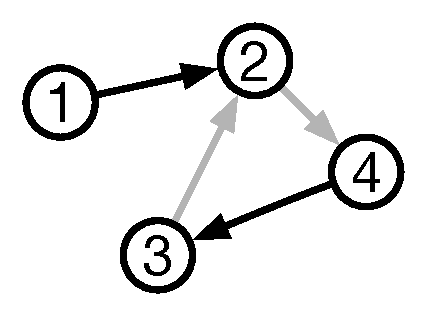
\includegraphics[height=3in]{imgs/example-graph.pdf}
          \caption{}
          \label{fig:sub1}
        \end{subfigure}%
        \hfill
        \begin{subfigure}{.43\textwidth}
          \centering
          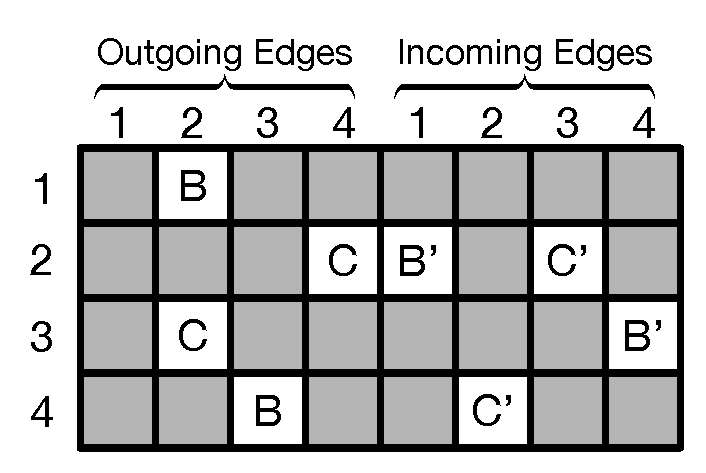
\includegraphics[height=3in]{imgs/recurrent-matrix-sparsity-pattern2.pdf}
          \caption{}
          \label{fig:sub2}
        \end{subfigure}
        \begin{subfigure}{.25\textwidth}
          \centering
          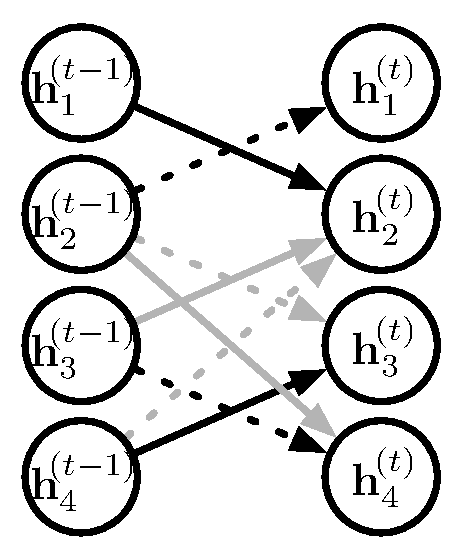
\includegraphics[height=3in]{imgs/unrolled-graph3.pdf}
          \caption{}
          \label{fig:sub2}
        \end{subfigure}
        
        \caption{(a) An example of a directed graph. Colour denotes the type of the edge. (b) Adjacency matrix with edge typing. (c) Message passing by unrolling recurrence for one timestep. Dotted lines denote propagation in reverse edge directions. This figure is a re-ordered duplicate of Figure 1 from \cite{DBLP:journals/corr/LiTBZ15}.}
        \label{fig:test}
      \end{figure}
      
      
    \end{block}
    
     \vspace{-0.6in} 
    \begin{block}{Gated Graph Neural Networks}
    We explain the mechanism implemented by a GGNN on a graph $\mathcal{G}=(\mathcal{V}, \mathcal{E})$, where $\mathcal{V}$ is the set of all the nodes, and $\mathcal{E}$ is the set of all the edges. Each node $v$ has annotations $x_v$. For an arbitrary directed edge from $u$ to $v$ of type $T$, we also include a directed edge from $v$ to $u$ of type $T'$ in $\mathcal{E}$.
    \vspace{0.2in}
    
    \textcolor{darkred}{Initialisation}\quad The latent representations for graph nodes are initialised by padding the node annotations:
    \begin{equation}
        \forall v \in \mathcal{V}. \quad \mathbf{h}_v^{0} = [\mathbf{x}_v^T, \mathbf{0}]^T.
    \end{equation}
    
    
    \textcolor{darkred}{Message Passing}\quad For an edge $u \to v$ of type $A$, let $\mathbf{h}_u^t$, $\mathbf{h}_v^t$ be the latent representations for $u$ and $v$ at the $t$-th step, and $\mathbf{A}, \mathbf{b}_A$ be the trainable edge type weight and bias associated with $A$. The message to pass from $u$ to $v$ is
    \begin{equation}
        \mathbf{m}_{uv}^t = \mathbf{A} \mathbf{h}_u^{t-1}.
    \end{equation}
    
    \textcolor{darkred}{Propagation}\quad At each iteration, each node representation is updated by combining messages from its neighbours and the latent representation from the last iteration:
    \begin{equation}
        \forall v \in \mathcal{V}. \quad \mathbf{h}_v^t = \textsc{GRU}\left(\mathbf{h}_v^{t-1}, 
         \mathbf{b} + add(\{\mathbf{m}_{uv}^t \mid (u, v) \in \mathcal{E} \})\right).
    \end{equation}
    \end{block}
    
    
    
    
  \end{column} % End of the 1st column

%%%%%%%%%%%%%%%%%%%%%%%%%%%%%%%%%%%%%%%%%%
%% Column 2
%%%%%%%%%%%%%%%%%%%%%%%%%%%%%%%%%%%%%%%%%%

  \begin{column}{.02\textwidth}\end{column} % Empty spacer column

  \begin{column}{.3\textwidth} % 2nd column
    % \vspace{\shrink}
    % \vspace{0.1in}
    
    \color{oxfordblue}
    \textcolor{darkred}{Output Modules} After $T$ iterations, the final latent representations for all the nodes are
    \begin{equation}
        \forall v \in \mathcal{V}.\quad \mathbf{s}_v = \mathbf{h}_v^T.
    \end{equation}
    
    An output module is used to obtain the appropriate output for each task. Two types of tasks are considered.
    \begin{itemize}
    \color{oxfordblue}
        \item Node selection. A differentiable scoring function $f_s$ and a softmax function are used to obtain a categorical distribution on nodes:
        \begin{equation}
            \mathbf{p}_{node} = \mathsf{softmax}\left(f_s([\mathbf{s}_{v_1}, \mathbf{s}_{v_2}, \ldots, \mathbf{s}_{v_{\mid \mathcal{V}\mid}}]^T)\right).
        \end{equation}
        \item Graph classification. A graph readout is first obtained for each graph $\mathcal{G}$:
        \begin{equation}
            \mathbf{h}_{\mathcal{G}} = \bigg(
                \displaystyle\sum_{v\in\mathcal{V}}  
                \sigma \left(f_1\left([\mathbf{s}_v^T, \mathbf{x}_v^T]^T\right)\right)
                \odot
                \tanh \left(f_2\left([\mathbf{s}_v^T, \mathbf{x}_v^T]^T\right)\right)
            \bigg),
        \end{equation}
        where $f_1$ and $f_2$ are both implemented by neural networks, $\sigma$ is the sigmoid function, $\tanh$ is the hyperbolic tangent function, and $\odot$ is element-wise production. Then a neural network function $f_c$ takes the graph readout and produces a probability vector over the classification categories:
        \begin{equation}
            \mathbf{p}_{\mathcal{G}} = \mathsf{softmax}\left(f_c\left(\mathbf{h}_{\mathcal{G}}\right)\right).
        \end{equation}
    \end{itemize}
    
    For a fixed number of recurrent unrolling steps, \textbf{GGNN is entirely differentiable. Gradients can be calculated by back propagation and back propagation through time.} $\implies$ a boost to optimisation. This was not the case for previous GNNs relying on contraction maps.
    
    
    \begin{block}{Gated Graph Sequence Neural Networks}
    GGNNs can take graphs as inputs and have a single output. To work with sequential outputs, a GGSNN is needed. Here, we explain the mechanism of a GGSNN with shared output and propagation modules producing an output sequence of length $L$.\vspace{0.2in}
    
    A schematic of the GGSNN architecture is shown in Figure \ref{fig:GGSNN}.
    \begin{figure}
        \centering
        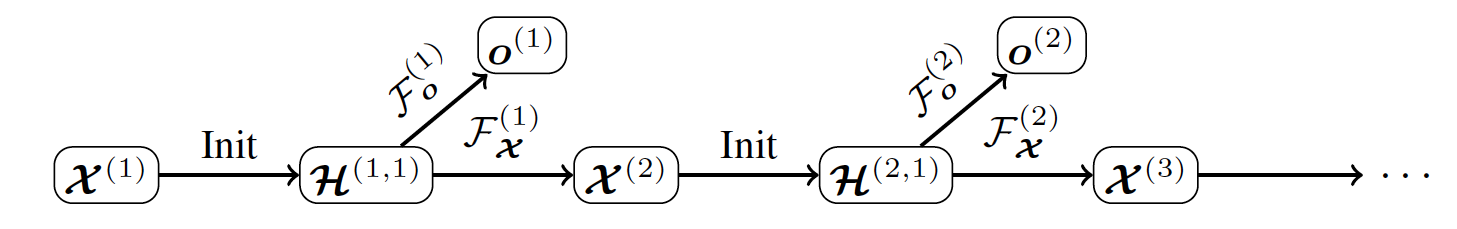
\includegraphics[width=\textwidth]{imgs/ggsnn.png}
        \caption{Diagram of the GGSNN mechanism. This is a duplicate of Figure 2 in \cite{DBLP:journals/corr/LiTBZ15}.}
        \label{fig:GGSNN}
    \end{figure}
    At each \textbf{Init} step, $\boldsymbol{\mathcal{X}}^{(l)}$ is padded with 0: $\boldsymbol{\mathcal{H}}^{(l, 1)} = [\boldsymbol{\mathcal{X}}^{(l)}, \boldsymbol{0}]$.
    Because we use a shared propagation model, we have $\mathcal{F}_{}^{(l)}$ and $\mathcal{F}_{\boldsymbol{\mathcal{X}}}^{(l)}$ to adopt the same GGNN layer $\mathcal{F}$ and have different output modules:
    
    \begin{equation}
    \begin{aligned}
        & \forall l \in [1, 2, \ldots, L].\quad \boldsymbol{H}^l = \boldsymbol{\mathcal{F}}\left(\boldsymbol{\mathcal{H}}^{(l, 1)}\right),\\
        & \boldsymbol{o}^{(l)} = 
        \boldsymbol{\mathcal{O}} \left(concat[\boldsymbol{H}^l, \boldsymbol{\mathcal{X}}^{(1)}]\right),
        \boldsymbol{\mathcal{X}}^{(l+1)} = \boldsymbol{\mathcal{P}}\left(concat[\boldsymbol{H}^l, \boldsymbol{\mathcal{X}}^{(1)}]\right),
    \end{aligned}
    \end{equation}
    where $\boldsymbol{\mathcal{O}}$ is an output module, and $\boldsymbol{\mathcal{P}}$ is a multi-layer perceptron for propagating information to the next prediction step.
    \vspace{0.2in}
    
    The loss can be calculated using the target sequence and the output sequence $[\boldsymbol{o}^{(1)}, \boldsymbol{o}^{(2)}, \ldots, \boldsymbol{o}^{(L)}]$
    
    \end{block}
    
    
    

  \end{column} % End of the 2nd column

%%%%%%%%%%%%%%%%%%%%%%%%%%%%%%%%%%%%%%%%%%
%% Column 3
%%%%%%%%%%%%%%%%%%%%%%%%%%%%%%%%%%%%%%%%%%

  \begin{column}{.02\textwidth}\end{column} % Empty spacer column
    
  \begin{column}{.3\textwidth} % 3rd column
  
  \vspace{\shrink}
    \begin{block}{Experiments}
      We contrasted the reproduced GGNNs and GGSNNs, as well as baseline recurrent neural networks, with the implementations in the paper~\cite{DBLP:journals/corr/LiTBZ15}, on a subset of bAbI tasks \cite{DBLP:journals/corr/WestonBCM15}. These tasks are bAbI task (4) Two argument relations, (15) Basic deduction, (16) Basic induction, (18) Size reasoning, and (19) Path finding. The tasks are represented in a symbolic logic form and converted to graphs for GGNNs and GGSNNs. The results are presented in Table \ref{table:table-1}.\vspace{0.1in}
      
      \begin{table}[t]
          \caption{Test accuracies~(in \%) of the models for selected bAbI tasks. Number in parentheses denotes the number of training examples required to reach the accuracy shown. Only the best highest accuracies of models and the minimum number of training examples to achieve them are shown.}\label{table:table-1}
          \vspace{0.1in}
          \centering
          \small
          \begin{tabular}{cccccc}
              \toprule
              bAbI Task & Implementation & RNN & LSTM & GGNN \\  \midrule
              \multirow{2}{*}{4} & Li et al. & $97.3 \pm 1.9\thinspace (250)$ & $97.4 \pm 2.0\thinspace  (250)$ & $\mathbf{100.0 \pm 0.0\thinspace (50)}$ \\
              & ours & $98.9 \pm 1.4\thinspace (250)$ & $96.6 \pm 2.5\thinspace (250)$ & $\mathbf{100.0 \pm 0.0\thinspace (50)}$ \\  \midrule
        
              \multirow{2}{*}{15} & Li et al. &  $48.6 \pm 1.9\thinspace (950)$ & $50.3 \pm 1.3\thinspace (950)$ & $\mathbf{100.0 \pm 0.0\thinspace (50)}$  \\
              & ours & $38.6 \pm 3.7\thinspace (950)$ & $49.9 \pm 0.7\thinspace (950)$ & $\mathbf{100.0 \pm 0.0\thinspace (50)}$ \\  \midrule
        
              \multirow{2}{*}{16} & Li et al. &  $33.0 \pm 1.9\thinspace (950)$&  $37.5 \pm 0.9\thinspace (950)$ & $\mathbf{100.0 \pm 0.0\thinspace (50)}$  \\
              & ours & $35.0 \pm 1.5\thinspace (950)$ & $39.0 \pm 0.9\thinspace (950)$ & $\mathbf{100.0 \pm 0.0\thinspace (50)}$ \\  \midrule
        
              \multirow{2}{*}{18} & Li et al. & $88.9 \pm 0.9\thinspace (950)$ & $88.9 \pm 0.8\thinspace (950)$ & $\mathbf{100.0 \pm 0.0\thinspace (50)}$ \\
              & ours & $89.6 \pm 0.4\thinspace (950)$ & $89.4 \pm 0.7\thinspace (950)$ & $99.6\pm 0.3\thinspace (500)$\\ \midrule
              
              bAbI Task & Implementation & RNN & LSTM & GGSNN \\  \midrule
              
              \multirow{2}{*}{19} & Li et al. & $24.7 \pm 2.7\thinspace (950)$ & $28.2 \pm 1.3\thinspace (950)$ & $99.0\pm1.1\thinspace (250)$\\ 
              & ours & $28.3 \pm 1.9\thinspace (950)$ & $29.7 \pm 1.8\thinspace (950)$ & $\mathbf{99.1\pm 0.8}\thinspace (500)$\\ \bottomrule
        \end{tabular}
        \end{table}
        \vspace{0.2in}
        
    \begin{itemize}
        \item \textcolor{darkred}{Reproducibility}\thinspace Given that the highest accuracies for each of the models matched very closely with those reported in the papaer, we consider the model as well as the bAbI experiments reproducible.
        \item \textcolor{darkred}{Difference in sample complexity}\thinspace Our models for tasks 18 and 19 have lower sample complexities since they need 500 training examples to reach the highest test accuracies, while the original implementation needs only 50 and 250, respectively.
    \end{itemize}
    \end{block}
    
    \begin{block}{Extensions}
    We extend the reproduction to answer three questions: (1) How important is the graph structure representation? (2) How important is the recurrent style of information processing? (3)
    \end{block}
    
    

    \begin{block}{References}
    %   \nocite{*} % Insert publications even if they are not cited in the poster
      \linespread{0.928}\selectfont
      \footnotesize{\bibliographystyle{unsrt}
      \bibliography{oxford_poster}}
    \end{block}
    
    

  \end{column} % End of the 3rd column

  \begin{column}{.02\textwidth}\end{column} % Empty spacer column

\end{columns} % End of all the columns in the poster

\end{frame} % End of the enclosing frame

\end{document}